
\qrchapter{https://forgottenpillar.com/rsc/en-fp-chapter12}{Ukweli wa mbinguni}

\emcap{Umbile la Mungu} unashughulikia ubora au hali ya Mungu kuwa Nafsi. Wakati wowote tunapoangalia kazi ya waanzilishi juu ya \emcap{Umbile la Mungu}, tunaona kwamba wote walikuwa katika upatano kwa mtazamo kwamba Mungu ni \textit{huluki} anayeshikika, mwenye mwili na viungo vyote. Tunaona kila wakati umoja wa ufikira na utafsiri, ambayo hutofautisha neno ‘\textit{roho}’ na neno ‘\textit{huluki}’. Kwa kutofautisha maneno haya, wanaeleza ubora au hali ya Mungu kuwa Nafsi\footnote{\href{https://www.merriam-webster.com/dictionary/personality}{Merriam-Webster Dictionary} inafafanua neno ‘\textit{personality}’ kama “\textit{ubora au hali ya kuwa Nafsi}”.}—\emcap{Umbile la Mungu}. Hitimisho zao zote zimefupishwa katika hoja ya kwanza ya \emcap{Kanuni za Msingi}. \others{Kuna \textbf{Mungu mmoja}, \textbf{nafsi} ya kibinafsi, ya kiroho, Muumba wa vitu vyote, muweza wa yote, mjuzi wa yote, … na \textbf{kila mahali anakuwepo kupitia mwakilishi wake, Roho Mtakatifu}. Zaburi 139:7.}[FPSDA 1.2][https://egwwritings.org/read?panels=p1299.6]

Kufikia sasa, katika kazi ya waanzilishi, tumeona kwamba \emcap{Umbile la Mungu} umeunganishwa kwa uthabiti na uhakika wa uwepo wa Mungu. Mungu ni huluki binafsi wa kiroho, mwenye mwili na umbo; hivyo, uwepo Wake unazuiliwa kwa eneo moja—kama Biblia inavyosema, katika hekalu Lake, Katika kiti chake Cha enzi ambapo amezungukwa na utukufu usioweza kukaribiwa. Lakini yuko kila mahali kupitia kwa Mwakilishi wake, Roho Mtakatifu. Ni wazi kwamba, Roho Mtakatifu ni roho, na si huluki, \bible{kwa maana roho haina nyama na mifupa kama mnionavyo mimi}, alisema Yesu (Luka 24:39). Kristo pia ni huluki, kama Baba Yake. Yeye ni taswira dhahiri ya Umbile wa Baba; kwa hiyo, Yeye huonyesha umbile sawa, au ubora au hali ya kuwa nafsi, kama Baba Yake.

Katika uzoefu wetu, tunapowasilisha imani za awali za Waadventista Wasabato juu ya \emcap{Umbile la Mungu} kwa ndugu zetu wa utatu, kama inavyoonyeshwa katika mambo mawili ya kwanza ya \emcap{Kanuni za Msingi}, mara nyingi wanadai kuwa kauli katika \emcap{Kanuni za Msingi} ni sahihi kwa njia fulani, lakini uelewaji unaohusishwa na maneno “\textit{Huluki binafsi wa kiroho}” ni uwongo. Kwa kawaida hujaribu kuoanisha \emcap{Kanuni za Msingi} na Fundisho la Utatu kwa kugeuza maneno “\textit{huluki wakiroho}”, kana kwamba neno ‘\textit{kiroho}’ linamaanisha jambo la ajabu, linalofaa kusawazisha \emcap{Umbile la Mungu} na wa Kristo na umbile la Roho Mtakatifu\footnote{Ubora au hali ya Roho Mtakatifu kuwa nafsi ni kutoa ushahidi, si kuwa na umbo la nafsi. \egw{\textbf{Roho Mtakatifu ana Nafsi}, \textbf{\underline{vinginevyo} Yeye asingeweza \underline{kutoa ushahidi} kwa roho zetu} na pamoja na roho zetu kwamba sisi ni watoto wa Mungu. \textbf{Lazima pia awe nafsi ya kiungu}, \textbf{\underline{vinginevyo} Yeye asingeweza \underline{kuchunguza} siri zilizofichika katika akili ya Mungu}. ‘Maana ni nani katika wanadamu ajuaye mambo ya binadamu ila roho ya binadamu iliyo ndani yake? Vivyo hivyo na mambo ya Mungu hakuna ayajuaye ila Roho wa Mungu.’ [1 Wakorintho 2:11.]}[21LtMs, Ms 20, 1906, par. 32][https://egwwritings.org/read?panels=p14071.10296041&index=0]. Ni wazi kabisa kwamba Roho Mtakatifu ni nafsi, lakini si kwa njia ile ile kama Baba na Mwana, kwani Roho Mtakatifu hana sifa ya umbo la nje la kimwili kama Baba na Mwana walivyo nalo.}. Tatizo la msingi linakuja kwenye uelewa wa Ukweli wa mbinguni. Biblia haiko kimya kuhusu mbingu na ukweli wake, na waanzilishi wetu walielewa vizuri. Hapa chini tunasoma kuhusu maelezo ya maneno “\textit{huluki wa kiroho}” kutoka James White na Uriah Smith katika kitabu chao, “\textit{The Biblical Institute}”. Biblia inaeleza haya maneno kwa kutumia mfano wa malaika, ambao ni “\textit{viumbe wa kiroho}”.

\begin{figure}[hp]
    \centering
    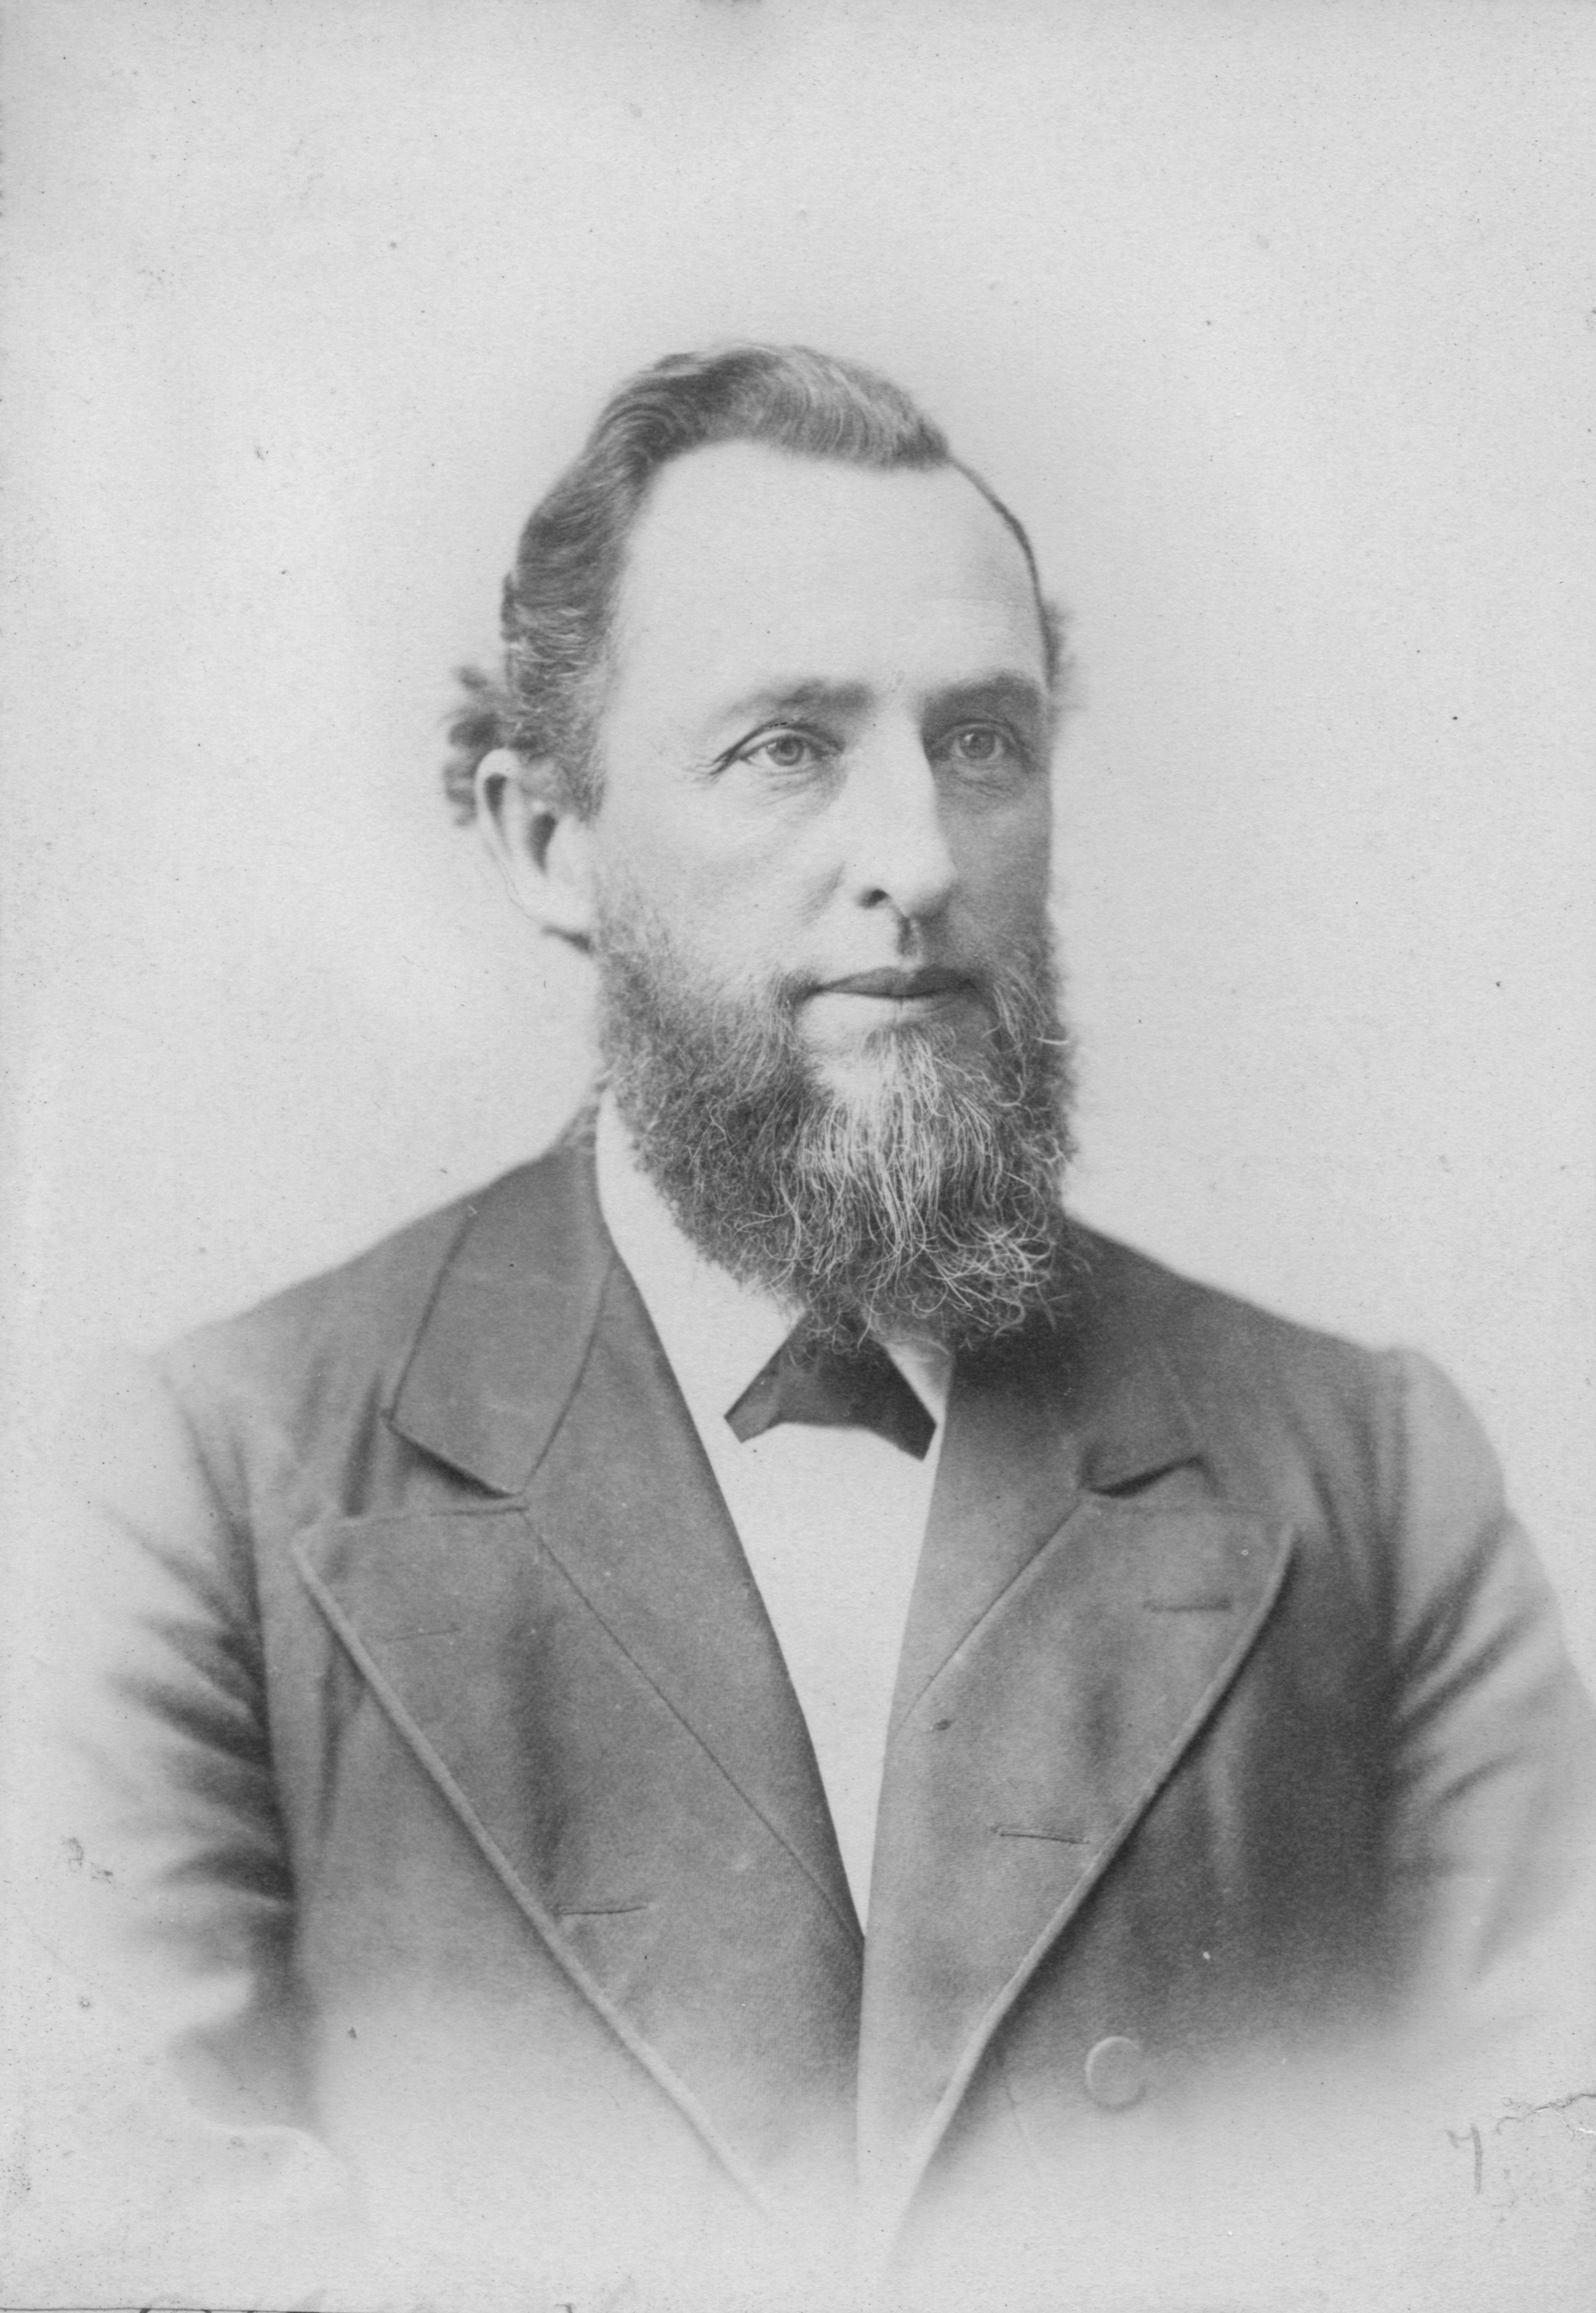
\includegraphics[width=1\linewidth]{images/uriah-smith.jpg}
    \caption*{Uriah Smith (1832-1903)}
    \label{fig:uriah-smith}
\end{figure}

\others{\textbf{Malaika ni viumbe halisi}. Wanaelezewa katika Biblia kuwa \textbf{wana uso, miguu, mabawa} \&x. Ezekieli asema hivi kuhusu makerubi, ‘\textbf{Mwili wao \underline{wote} na migongo yao na mikono yao na mbawa zao},’ \&c. Eze. 10:12. Malaika \textbf{walimtokea} Ibrahimu. Mwanzo 18:1-8. Walizungumza na kula naye. Wakaenda Sodoma na kuzungumza na Loti, ambaye, akiingia nyumbani kwake akawapikia mikate isiyotiwa chachu, nao wakala. \textbf{Nafsi hawa waliitwa malaika}. Daudi anazungumza juu ya mana kama nafaka ya Mbinguni na chakula cha malaika. Zab. 78:23-25.}

\othersnogap{Kesi ya Balaamu, Hes. 22:22-31, ni tukio la kuvutia. Malaika \textbf{alimtokea} Balaamu akiwa na upanga \textbf{mkononi mwake}. Swali wakati mwingine huulizwa \textbf{jinsi malaika wanaweza kuwa viumbe vya kimwili kwa vile \underline{hatuwezi kuwaona}. Kesi hii inadhihirisha}. Rekodi inasema \textbf{Bwana alimfumbua macho Balaamu akamwona yule malaika}. \textbf{Malaika hakuunda mwili kwa hafla hiyo}. \textbf{Alikuwa vile vile tu alivyokuwa kabla Balaamu kumwona; lakini \underline{badiliko likatukia katika Balaamu}}. Macho yake yakafumbuliwa, kisha akawaona malaika. Ndivyo ilivyokuwa na mtumishi wa Elisha wakati yeye na bwana wake walipoletwa mahali pazuri pa wakizungukwa na jeshi la mfalme wa Shamu. 2 Wafalme 6:17. Elisha aliomba ili \textbf{macho ya mtumishi wake yafumbuliwe}; na mara hiyo akaona mlima wote ulikiwa umejaa farasi na magari ya vita kumzunguka Elisha.}

\othersnogap{\textbf{Hii inaweza kuonyeshwa zaidi ikirejelea vitu ambavyo tunajua ni vyenye dutu na bado ambayo hatuwezi kuona}. Hewa ni dutu, mwanga ni dutu, hata mawazo yenyewe ni matokeo tu ya mashirika ya dutu — dutu linalofanya kazi juu ya dutu — na bado hatuwezi kuona haya mambo. \textbf{Vivyo hivyo na malaika}.}

\othersnogap{\textbf{Inapingwa zaidi juu ya maumbile ya malaika kwamba wanaitwa roho.} Ebr. 1:13, 14. \textbf{\underline{Lakini hili si pingamizi kwa wao kuwa viumbe halisi}}. \textbf{Wao ni viumbe tu wa kiroho waliopangwa tofauti na miili hii ya duniani tuliyo nayo}. Paulo anasema, 1 Kor. 15:44, ‘\textbf{Kuna mwili wa asili na kuna \underline{mwili wa kiroho}}.’ \textbf{Mwili wa asili tunao Sasa; ilhali mwili wa kiroho tutakuwa nao katika ufufuo}. ‘\textbf{Unafufuliwa mwili wa kiroho}.’ Aya 44. \textbf{Lakini basi sisi ni sawa na malaika}, Lk 20:36; \textbf{kwa kuwa tuna miili kama mwili wa Kristo mtukufu zaidi}. Fil. 3:4\footnote{Typo: Inapaswa kuwa Wafilipi 3:21} \textbf{naye Kristo si Roho kiasi na malaika}. \textbf{Tunasoma kwamba Mungu ni roho, yaani, \underline{huluki wa kiroho tu}}.}[James White and Uriah Smith, The Biblical Institute (Kindle Locations 2537-2553). Kindle Edition.]

Biblia inatupa ufahamu kwamba malaika ni viumbe vya kiroho vilivyo na miili ya kimwili, lakini bado hawaonekani kwetu, isipokuwa Bwana atufungue macho tuwaone. Wakati wenye haki watainuka katika miili yao mipya yenye utukufu, watafufuka katika mwili wa kiroho, usioharibika. Mwili huu utakuwa wa kushikika na wenye uliopo kama vile Dunia mpya itakuwa ya kushikika na yenye iliopo. Na kwa miili yetu ya kiroho tutamiliki Dunia iliyofanywa upya, tutaijaza \bible{na kuitawala na muwe na mamlaka juu ya samaki wa baharini, na ndege wa angani, na juu ya kila kiumbe chenye uhai kiendacho juu ya nchi}[Mwanzo 1:28].

% Heaven's reality

\begin{titledpoem}
    
    \stanza{
        God is not vapor, nor mystery unknown, \\
        A personal being upon Heaven's throne. \\
        Bound by space as a being must, \\
        Yet present through His Spirit's trust.
    }

    \stanza{
        Christ bears His image, a tangible Son, \\
        Two divine beings, not mystically one. \\
        Angels around them with bodies unseen, \\
        Material creatures of heavenly sheen.
    }

    \stanza{
        Our eyes cannot witness their spiritual frame, \\
        Until God reveals what our vision can't claim. \\
        In resurrection we'll rise like them too, \\
        Spiritual bodies, yet tangible and true.
    }

    \stanza{
        Not three equal persons in mystical blend, \\
        But Father and Son with Spirit they send. \\
        The divine is not distant, abstract, or obscure, \\
        But personal, present, and perfectly sure.
    }
    
\end{titledpoem}

Ukweli wa mbinguni
